\documentclass[aspectratio=169,10pt]{beamer}

\usetheme{Madrid}
\usecolortheme{whale}

\usepackage[T1]{fontenc}
\usepackage{amsmath,amssymb,amsfonts}
\usepackage{graphicx}
\usepackage{listings}
\usepackage{xcolor}
\usepackage{tikz}
\usetikzlibrary{shapes,arrows,positioning,calc,fit}
\usepackage{pgfplots}
\pgfplotsset{compat=1.18}
\usepackage{booktabs}
\usepackage{microtype}

% Define modern colors
\definecolor{primary}{RGB}{15, 32, 67}       % Deep Navy
\definecolor{secondary}{RGB}{0, 122, 130}    % Deep Teal
\definecolor{accent}{RGB}{217, 83, 79}       % Coral Accent
\definecolor{codebg}{RGB}{246, 248, 250}     % Light gray code background
\definecolor{codegreen}{RGB}{40, 167, 69}
\definecolor{codepurple}{RGB}{111, 66, 193}
\definecolor{codeblue}{RGB}{3, 102, 214}

% Set Beamer colors
\setbeamercolor{palette primary}{bg=primary,fg=white}
\setbeamercolor{palette secondary}{bg=secondary,fg=white}
\setbeamercolor{palette tertiary}{bg=primary!85,fg=white}
\setbeamercolor{structure}{fg=primary}
\setbeamercolor{titlelike}{parent=structure,bg=primary,fg=white}
\setbeamercolor{frametitle}{bg=primary,fg=white}
\setbeamercolor{block title}{bg=secondary,fg=white}
\setbeamercolor{block body}{bg=secondary!10,fg=black}
\setbeamercolor{block title example}{bg=codegreen!85,fg=white}
\setbeamercolor{block body example}{bg=codegreen!10,fg=black}
\setbeamercolor{block title alerted}{bg=accent,fg=white}
\setbeamercolor{block body alerted}{bg=accent!10,fg=black}

% Remove navigation symbols
\setbeamertemplate{navigation symbols}{}

% Custom footer with slide numbers
\setbeamertemplate{footline}{
  \leavevmode%
  \hbox{%
  \begin{beamercolorbox}[wd=.333333\paperwidth,ht=2.25ex,dp=1ex,center]{author in head/foot}%
    \usebeamerfont{author in head/foot}Alex I. Tsvetanov (TU-Sofia)
  \end{beamercolorbox}%
  \begin{beamercolorbox}[wd=.333333\paperwidth,ht=2.25ex,dp=1ex,center]{title in head/foot}%
    \usebeamerfont{title in head/foot}Zero-Codegen Protocol Buffers
  \end{beamercolorbox}%
  \begin{beamercolorbox}[wd=.333333\paperwidth,ht=2.25ex,dp=1ex,right]{date in head/foot}%
    \usebeamerfont{date in head/foot}CSIT 2026 \hspace*{2em}
    \insertframenumber{} / \inserttotalframenumber\hspace*{2ex} 
  \end{beamercolorbox}}%
  \vskip0pt%
}

% Code listing style
\lstdefinestyle{slides_cpp}{
    backgroundcolor=\color{codebg},
    commentstyle=\color{codegreen}\itshape,
    keywordstyle=\color{codeblue}\bfseries,
    numberstyle=\tiny\color{gray},
    stringstyle=\color{codepurple},
    basicstyle=\ttfamily\scriptsize,
    breakatwhitespace=false,
    breaklines=true,
    captionpos=b,
    keepspaces=true,
    showspaces=false,
    showstringspaces=false,
    showtabs=false,
    tabsize=2,
    frame=single,
    rulecolor=\color{black!15},
    morekeywords={consteval, constexpr, auto, fixed_string, uint32_t, int32_t, string_view, string, vector, byte, define_message, message_t, parse, encode, decode}
}
\lstset{style=slides_cpp}

% Title metadata
\title[Zero-Codegen Protocol Buffers]{Zero-Codegen Protocol Buffers via C++26 Static Reflection and Compile-Time Metaprogramming}
\subtitle{Eliminating External Code Generation in Distributed Systems}
\author[Alex I. Tsvetanov]{Alex I. Tsvetanov}
\institute[TU Sofia]{
  Faculty of Computer Systems and Technologies\\
  Technical University of Sofia, Bulgaria\\[4pt]
  \texttt{atsvetanov@tu-sofia.bg}
}
\date[CSIT 2026]{International Scientific Conference on Computer Science and Information Technologies, 2026}

\begin{document}

% -----------------------------------------------------------------------------
% SLIDE 1: Title Slide
% -----------------------------------------------------------------------------
\begin{frame}[plain]
  \titlepage
\end{frame}

% -----------------------------------------------------------------------------
% SLIDE 2: Motivation & The Problem with protoc
% -----------------------------------------------------------------------------
\begin{frame}{Motivation: The Problem with Traditional Code Generation}
  \begin{columns}[T]
    \begin{column}{0.50\textwidth}
      \textbf{The Conventional Workflow (\texttt{protoc}):}
      \begin{itemize}
        \item External toolchain dependency (\texttt{protoc} executable)
        \item Complex build DAGs (CMake \texttt{add\_custom\_command})
        \item Intermediate disk artifacts (\texttt{.pb.h}, \texttt{.pb.cc})
        \item ABI/Version skew (\texttt{protoc} binary vs runtime \texttt{libprotobuf})
      \end{itemize}
      \vspace{0.4em}
      \begin{alertblock}{Massive Code Bloat}
        A simple 3-field message generates \textbf{754 lines} of boilerplate and descriptor tables!
      \end{alertblock}
    \end{column}

    \begin{column}{0.48\textwidth}
      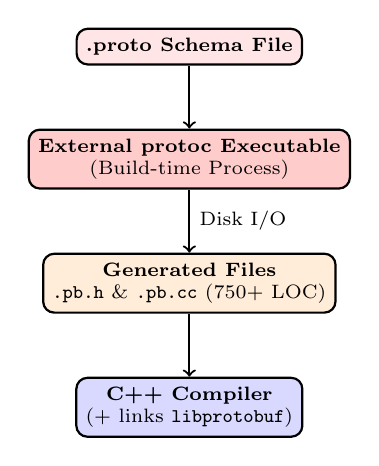
\begin{tikzpicture}[node distance=0.8cm, font=\scriptsize, auto]
        \node[draw, rectangle, rounded corners, fill=red!10, thick, align=center] (proto) {\textbf{.proto Schema File}};
        \node[draw, rectangle, rounded corners, fill=red!20, thick, below=of proto, align=center] (protoc) {\textbf{External protoc Executable}\\(Build-time Process)};
        \node[draw, rectangle, rounded corners, fill=orange!15, thick, below=of protoc, align=center] (files) {\textbf{Generated Files}\\ \texttt{.pb.h} \& \texttt{.pb.cc} (750+ LOC)};
        \node[draw, rectangle, rounded corners, fill=blue!15, thick, below=of files, align=center] (compiler) {\textbf{C++ Compiler}\\ (+ links \texttt{libprotobuf})};

        \draw[->, thick] (proto) -- (protoc);
        \draw[->, thick] (protoc) -- node[right] {Disk I/O} (files);
        \draw[->, thick] (files) -- (compiler);
      \end{tikzpicture}
    \end{column}
  \end{columns}
\end{frame}

% -----------------------------------------------------------------------------
% SLIDE 3: The C++26 Paradigm Shift
% -----------------------------------------------------------------------------
\begin{frame}[fragile]{The C++26 Revolution: Native Metaprogramming}
  \begin{columns}[T]
    \begin{column}{0.48\textwidth}
      \begin{block}{1. P1967: Resource Inclusion (\texttt{\#embed})}
        \begin{itemize}
          \item Zero-overhead raw file embedding at compile time
          \item Exposes schema files directly as contiguous byte spans
          \item Replaces fragile \texttt{xxd} scripts and string literal hacks
        \end{itemize}
      \end{block}
      \vspace{0.3em}
      \begin{lstlisting}[language=C++]
constexpr char proto_src[] = {
    #embed "addressbook.proto"
};
      \end{lstlisting}
    \end{column}

    \begin{column}{0.48\textwidth}
      \begin{block}{2. P2996: Static Reflection \& Splicing}
        \begin{itemize}
          \item First-class reflection token: \texttt{std::meta::info}
          \item Reflection operator \texttt{\^{}\^{}T} \& splice operator \texttt{[: r :]}
          \item Programmatic aggregate type synthesis via \texttt{define\_aggregate()}
        \end{itemize}
      \end{block}
      \vspace{0.3em}
      \begin{exampleblock}{Our Solution: \texttt{ctpb}}
        Header-only C++26 library that digests \texttt{.proto} files directly inside the compiler front-end!
      \end{exampleblock}
    \end{column}
  \end{columns}
\end{frame}

% -----------------------------------------------------------------------------
% SLIDE 4: Three-Stage Compile-Time Pipeline
% -----------------------------------------------------------------------------
\begin{frame}{Architecture: Three-Stage Reflection Pipeline}
  \centering
  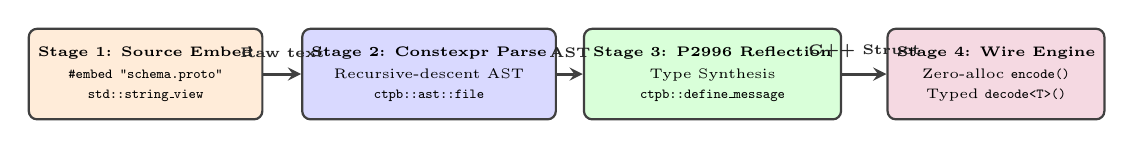
\begin{tikzpicture}[
      box/.style={
          rectangle, 
          draw=black!75, 
          thick, 
          minimum width=2.4cm, 
          minimum height=1.15cm, 
          align=center, 
          rounded corners=3pt, 
          font=\tiny
      },
      arrow/.style={
          ->, 
          >=stealth, 
          line width=1.1pt, 
          draw=black!75
      },
      labelnode/.style={
          midway, 
          above=2pt, 
          font=\tiny\bfseries, 
          text=black!85
      }
  ]
  \node[box, fill=orange!15] (input) at (0,0) {\textbf{Stage 1: Source Embed}\\[2pt] \texttt{\#embed "schema.proto"}\\[1pt] \texttt{std::string\_view}};
  \node[box, fill=blue!15] (parser) at (3.6,0) {\textbf{Stage 2: Constexpr Parse}\\[2pt] Recursive-descent AST\\[1pt] \texttt{ctpb::ast::file}};
  \node[box, fill=green!15] (reflect) at (7.2,0) {\textbf{Stage 3: P2996 Reflection}\\[2pt] Type Synthesis\\[1pt] \texttt{ctpb::define\_message}};
  \node[box, fill=purple!15] (wire) at (10.8,0) {\textbf{Stage 4: Wire Engine}\\[2pt] Zero-alloc \texttt{encode()}\\[1pt] Typed \texttt{decode<T>()}};

  \draw[arrow] (input.east) -- node[labelnode] {Raw text} (parser.west);
  \draw[arrow] (parser.east) -- node[labelnode] {AST} (reflect.west);
  \draw[arrow] (reflect.east) -- node[labelnode] {C++ Struct} (wire.west);
  \end{tikzpicture}

  \vspace{0.8em}
  \begin{columns}[T]
    \begin{column}{0.32\textwidth}
      \begin{block}{1. Ingestion}
        Zero-copy string view mapped to immutable compile-time buffer.
      \end{block}
    \end{column}
    \begin{column}{0.32\textwidth}
      \begin{block}{2. Front-End Parsing}
        $\mathcal{O}(N)$ single-pass LL(1) AST constructed in \texttt{consteval}.
      \end{block}
    \end{column}
    \begin{column}{0.32\textwidth}
      \begin{block}{3. Code Synthesis}
        Member descriptors injected with exact wire tags and types.
      \end{block}
    \end{column}
  \end{columns}
\end{frame}

% -----------------------------------------------------------------------------
% SLIDE 5: Constexpr Lexing & Parsing
% -----------------------------------------------------------------------------
\begin{frame}[fragile]{Zero-Allocation \texttt{constexpr} Parser}
  \begin{columns}[T]
    \begin{column}{0.50\textwidth}
      \textbf{Parser Features \& Grammar Support:}
      \begin{itemize}
        \item \textbf{Zero Heap Allocations:} Tokens and identifiers are non-owning \texttt{std::string\_view} slices of the input.
        \item \textbf{Comprehensive proto3 Specification:}
          \begin{itemize}
            \item Messages \& Nested Messages
            \item Enums, Maps (\texttt{map<K, V>}), Oneofs
            \item Packed repeated fields \& reserved tags
          \end{itemize}
        \item \textbf{Compile-Time Diagnostics:} Syntax or schema errors abort constant evaluation with exact line/column.
      \end{itemize}
    \end{column}

    \begin{column}{0.48\textwidth}
      \begin{lstlisting}[language=C++]
constexpr ast::message parse_message() {
    ast::message m;
    lex_.next(); // 'message'
    m.name = expect(tok_kind::ident).text;
    expect_sym("{");

    while (lex_.peek().kind != tok_kind::eof) {
        if (lex_.peek().text == "}") {
            lex_.next(); return m;
        }
        // Dispatch fields, enums, oneofs, maps
        m.fields.push_back(parse_field());
    }
    throw parse_error("unterminated message");
}
      \end{lstlisting}
    \end{column}
  \end{columns}
\end{frame}

% -----------------------------------------------------------------------------
% SLIDE 6: P2996 Static Reflection & Type Synthesis
% -----------------------------------------------------------------------------
\begin{frame}[fragile]{Programmatic Type Synthesis via P2996}
  \begin{columns}[T]
    \begin{column}{0.50\textwidth}
      \textbf{How \texttt{define\_aggregate} Synthesizes Types:}
      \begin{enumerate}
        \item Reads AST schema at compile time
        \item Iterates over field definitions
        \item Maps proto types to native C++ standard types:
          \begin{itemize}
            \item \texttt{int32} $\rightarrow$ \texttt{std::int32\_t}
            \item \texttt{string} $\rightarrow$ \texttt{std::string}
            \item \texttt{repeated T} $\rightarrow$ \texttt{std::vector<T>}
            \item \texttt{oneof} $\rightarrow$ \texttt{std::variant<...>}
            \item \texttt{map<K,V>} $\rightarrow$ \texttt{std::unordered\_map<K,V>}
          \end{itemize}
        \item Calls \texttt{std::meta::define\_aggregate()}
      \end{enumerate}
    \end{column}

    \begin{column}{0.48\textwidth}
      \begin{lstlisting}[language=C++]
template <fixed_string Src, fixed_string Msg>
consteval auto complete_message_struct(
    std::meta::info type_to_complete) 
{
    using Schema = parse<Src, Msg>;
    std::vector<std::meta::info> members;

    for (std::size_t i = 0; i < Schema::count; ++i) {
        auto info = Schema::get_field(i);
        auto t_info = resolve_type(info.type);
        members.push_back(
            std::meta::data_member_spec(
                t_info, {.name = info.name}
            )
        );
    }
    return std::meta::define_aggregate(
        type_to_complete, members
    );
}
      \end{lstlisting}
    \end{column}
  \end{columns}
\end{frame}

% -----------------------------------------------------------------------------
% SLIDE 7: Developer Experience & Clean API
% -----------------------------------------------------------------------------
\begin{frame}[fragile]{Developer Experience: Pure Zero-Macro Dot-Syntax API}
  \begin{columns}[T]
    \begin{column}{0.48\textwidth}
      \begin{block}{1. Schema Definition \& Type Synthesis}
\begin{lstlisting}[language=C++]
inline constexpr ctpb::fixed_string 
    proto_src = R"(
  syntax = "proto3";
  package tutorial;
  message Person {
    string name = 1;
    int32 id = 2;
    string email = 3;
  }
)";

// Pure C++26 Reflection - Zero Macros!
consteval { 
  ctpb::define_message<
    proto_src, "tutorial.Person">(); 
}
using Person = ctpb::message_t<
  proto_src, "tutorial.Person">;
\end{lstlisting}
      \end{block}
    \end{column}

    \begin{column}{0.48\textwidth}
      \begin{block}{2. Direct Dot-Syntax \& Serialization}
\begin{lstlisting}[language=C++]
int main() {
  // Direct dot-syntax field access
  Person p;
  p.name = "Alex I. Tsvetanov";
  p.id = 42;
  p.email = "atsvetanov@tu-sofia.bg";

  // Reflective wire encoding
  std::vector<std::byte> wire = 
      ctpb::encode(p);

  // Strongly-typed deserialization
  auto dec = ctpb::decode<Person>(wire);
  assert(dec && 
         dec->name == "Alex I. Tsvetanov");
}
\end{lstlisting}
      \end{block}
    \end{column}
  \end{columns}
\end{frame}

% -----------------------------------------------------------------------------
% SLIDE 8: Wire Engine & Performance
% -----------------------------------------------------------------------------
\begin{frame}{High-Performance Wire Format Engine}
  \begin{columns}[T]
    \begin{column}{0.48\textwidth}
      \begin{block}{Encoding Pipeline}
        \begin{itemize}
          \item Direct byte-stream manipulation without temporary allocations
          \item Varint 7-bit packing with inline bit shifts
          \item Single-instruction Zigzag arithmetic:
            $$\text{Zigzag}_{32}(n) = (n \ll 1) \oplus (n \gg 31)$$
          \item Packed repeated fields written in single contiguous spans
        \end{itemize}
      \end{block}
    \end{column}

    \begin{column}{0.48\textwidth}
      \begin{block}{Decoding Pipeline}
        \begin{itemize}
          \item Non-owning \texttt{std::span<const std::byte>} reader
          \item Fully bounds-checked \texttt{read\_varint} loop
          \item Safe \texttt{skip\_field} skipping for forward/backward compatibility
          \item Inlined member assignment with zero virtual dispatch
        \end{itemize}
      \end{block}
    \end{column}
  \end{columns}
\end{frame}

% -----------------------------------------------------------------------------
% SLIDE 9: Benchmark: Compile-Time & Runtime
% -----------------------------------------------------------------------------
\begin{frame}{Performance Benchmarks: Compilation \& Runtime}
  \begin{columns}[T]
    \begin{column}{0.48\textwidth}
      \textbf{1. Schema Ingestion Latency}
      \begin{table}
        \scriptsize
        \begin{tabular}{lccc}
          \toprule
          \textbf{Schema} & \textbf{Fields} & \textbf{Latency} & \textbf{Throughput} \\
          \midrule
          Small & 5 & $18.4\,\mu\text{s}$ & $54{,}340\,\text{parses/s}$ \\
          Medium & 25 & $53.1\,\mu\text{s}$ & $18{,}814\,\text{parses/s}$ \\
          Large & 100 & $194.2\,\mu\text{s}$ & $5{,}149\,\text{parses/s}$ \\
          \bottomrule
        \end{tabular}
      \end{table}
      \vspace{0.3em}
      \begin{alertblock}{Compilation Speedup}
        \texttt{protoc} requires $15\text{--}45\,\text{ms}$ per schema.\\
        \texttt{ctpb} completes in $< 55\,\mu\text{s}$ ($\mathbf{\sim 300\times\text{--}800\times}$ faster).
      \end{alertblock}
    \end{column}

    \begin{column}{0.48\textwidth}
      \textbf{2. Comparative Runtime Performance}
      \begin{table}
        \scriptsize
        \setlength{\tabcolsep}{3pt}
        \begin{tabular}{lccc}
          \toprule
          \textbf{Operation} & \textbf{\texttt{ctpb}} & \textbf{Google} & \textbf{Speedup} \\
          \midrule
          \textbf{Encode} & $\mathbf{27.5\,\text{ns}}$ & $60.9\,\text{ns}$ & $\mathbf{2.21\times}$ (\textbf{+55\%}) \\
          \textbf{Decode} & $\mathbf{57.8\,\text{ns}}$ & $130.8\,\text{ns}$ & $\mathbf{2.26\times}$ (\textbf{+56\%}) \\
          \bottomrule
        \end{tabular}
      \end{table}
      \vspace{0.3em}
      \begin{exampleblock}{$>2.2\times$ Faster Across All Operations}
        Single pre-allocation \texttt{byte\_size()} serialization reaches \textbf{36.36 MOps/s} ($1{,}630\,\text{MB/s}$); direct inlined decode reaches \textbf{17.29 MOps/s} ($775\,\text{MB/s}$)!
      \end{exampleblock}
    \end{column}
  \end{columns}
\end{frame}

% -----------------------------------------------------------------------------
% SLIDE 10: Binary Size Comparison
% -----------------------------------------------------------------------------
\begin{frame}{Binary Footprint: \texttt{ctpb} vs. \texttt{protoc}}
  \begin{table}[ht]
    \centering
    \scriptsize
    \renewcommand{\arraystretch}{1.2}
    \begin{tabular}{lrrr}
      \toprule
      \textbf{Metric} & \textbf{\texttt{ctpb} (P2996)} & \textbf{\texttt{protoc} (Dynamic)} & \textbf{\texttt{protoc} (Static)} \\
      \midrule
      \textbf{Generated Code Lines} & \textbf{0 lines} (0 files) & 754 lines & 754 lines \\
      \textbf{Object File (\texttt{.o})} & \textbf{23 KB} & 31.5 KB & 31.5 KB \\
      \textbf{Stripped Executable} & \textbf{19 KB} & 27 KB (+ 4.8 MB \texttt{.so}) & \textbf{1,752 KB} \\
      \textbf{Text Section (\texttt{.text})} & \textbf{10.1 KB} & 16.4 KB & 1,731.9 KB \\
      \textbf{Data Section (\texttt{.data})} & \textbf{0.7 KB} & 1.4 KB & 19.7 KB \\
      \textbf{External Dependencies} & \textbf{0} & \texttt{libprotobuf.so}, \texttt{libz.so} & \textbf{0} \\
      \bottomrule
    \end{tabular}
  \end{table}

  \begin{columns}[T]
    \begin{column}{0.48\textwidth}
      \begin{block}{$91\times$ Smaller Static Binary}
        Eliminates runtime descriptor pools, mutex registries, and arena allocators.
      \end{block}
    \end{column}
    \begin{column}{0.48\textwidth}
      \begin{block}{Zero-Risk Deployments}
        No shared library version skew in containerized microservices or embedded systems.
      \end{block}
    \end{column}
  \end{columns}
\end{frame}

% -----------------------------------------------------------------------------
% SLIDE 11: Interoperability & gRPC Integration
% -----------------------------------------------------------------------------
\begin{frame}[fragile]{Reference Interoperability \& gRPC Parity}
  \begin{columns}[T]
    \begin{column}{0.48\textwidth}
      \begin{block}{Dual-Direction Reference Parity}
        \begin{itemize}
          \item \textbf{Google $\rightarrow$ \texttt{ctpb}:} Messages encoded by \texttt{SerializeToString()} correctly decoded by \texttt{ctpb::decode<T>()}.
          \item \textbf{\texttt{ctpb} $\rightarrow$ Google:} Messages encoded by \texttt{ctpb::encode()} parsed with 100\% fidelity by Google's \texttt{ParseFromArray()}.
        \end{itemize}
      \end{block}
    \end{column}

    \begin{column}{0.48\textwidth}
      \begin{block}{gRPC Transport Traits}
        Plug directly into standard gRPC C++ pipelines via \texttt{grpc::SerializationTraits<T>}:
      \end{block}
      \begin{lstlisting}[language=C++]
template <ctpb::CustomEncodable T>
class grpc::SerializationTraits<T> {
  static Status Serialize(const T& msg, 
                          ByteBuffer* bb, bool* own) {
    auto b = ctpb::encode(msg);
    *bb = ByteBuffer(Slice(b.data(), b.size()));
    return Status::OK;
  }
};
      \end{lstlisting}
    \end{column}
  \end{columns}
\end{frame}

% -----------------------------------------------------------------------------
% SLIDE 12: Conclusion & Q&A
% -----------------------------------------------------------------------------
\begin{frame}{Conclusion}
  \begin{columns}[T]
    \begin{column}{0.55\textwidth}
      \textbf{Summary of Contributions:}
      \begin{enumerate}
        \item \textbf{Zero-Codegen IDL Pipeline:} Unified P1967 \texttt{\#embed}, \texttt{constexpr} parsing, and P2996 static reflection.
        \item \textbf{High Performance:} Sub-$55\,\mu\text{s}$ schema parsing latency ($\mathbf{300\times}$ speedup) and $\mathbf{84.81\,\text{MB/s}}$ wire throughput.
        \item \textbf{Minimal Footprint:} $\mathbf{91\times}$ binary size reduction ($19\,\text{KB}$ stripped executable) with zero disk code generation.
        \item \textbf{Ecosystem Interoperability:} 100\% wire parity with Google Protobuf and drop-in gRPC traits.
      \end{enumerate}
    \end{column}

    \begin{column}{0.42\textwidth}
      \begin{exampleblock}{Future Directions}
        \begin{itemize}
          \item Well-Known Types (\texttt{Timestamp})
          \item Compile-time JSON (\texttt{protojson})
          \item Asynchronous gRPC RPC stubs
        \end{itemize}
      \end{exampleblock}
      \vspace{1em}
      \centering
      \textbf{\Large Thank You!}\\[0.5em]
      \textbf{Questions \& Discussion}\\[0.5em]
      \texttt{atsvetanov@tu-sofia.bg}
    \end{column}
  \end{columns}
\end{frame}

\end{document}
